\title{CS303 : DataBases and Information Systems\\
    \vspace{0.6cm}
    Assignment 2 
} % You may change the title if you want.
% \subtitle{Hello}
\author{Sourabh Bhosale \\ 200010004}

\date{\today}

\documentclass[12pt]{article}
\usepackage{fullpage}
\usepackage{enumitem}
\usepackage{amsmath,mathtools}
\usepackage{amssymb}
\usepackage[super]{nth}
\usepackage{textcomp}
\usepackage{hyperref}
\usepackage{multicol}
\usepackage{multirow}
\usepackage{minted}
% \usepackage{fontspec}
% \usepackage[showframe]{geometry}

% \usepackage[default,oldstyle,scale=0.95]{helvet}
% \usepackage[T1]{fontenc}

% \usepackage{merriweather}
% \usepackage[T1]{fontenc}

% \usepackage[sfdefault]{noto}
% \usepackage[T1]{fontenc}

\usepackage[default,oldstyle,scale=0.95]{opensans} %% Alternatively
%% use the option 'defaultsans' instead of 'default' to replace the
%% sans serif font only.
\usepackage[T1]{fontenc}

% \usepackage[scaled]{helvet} 
% \setmainfont{Roboto}
\usepackage{titling}
\hypersetup{
    colorlinks=true,
    linkcolor=blue,
    filecolor=magenta,      
    urlcolor=cyan,
}

\renewcommand\maketitlehooka{\null\mbox{}\vfill}
\renewcommand\maketitlehookd{\vfill\null}

\begin{document}


\begin{titlingpage}
\maketitle
\end{titlingpage}

\newpage
%---------------------------------------------------------------------

% \begin{tiny}
\section{Problem 1}

\subsection*{Suppose that we have relation marks(ID, score) and we wish to assign grades to students based on the score as follows : grade F if score $<$ 40, grade C if 40 $\leq$ score $<$ 60, grade B if 60 $\leq$ score $<$ 80, and grade A if 80 $\leq$ score. Write SQL queries to do the following :}

\subsubsection*{(a) Display the grade for each student, based on the marks relation.}

If we want to update the original table, then first approach does that. 
\vspace{5mm} \\
\fbox{ 
    \begin{minipage}{40em}
    \inputminted{mysql}{src/1a_a1.sql}
    \end{minipage}
}
\vspace{5mm} \\
If we don't want to update the original table, then second approach does that. 
\vspace{5mm} \\
\fbox{ 
    \begin{minipage}{40em}
    \inputminted{mysql}{src/1a_a2.sql}
    \end{minipage}
}
\subsubsection*{(b) Find the number of students with each grade.}

\fbox{ 
    \begin{minipage}{40em}
    \inputminted{mysql}{src/1b.sql}
    \end{minipage}
}

\newpage
%---------------------------------------------------------------------

\section{Problem 2}

\subsection*{Write SQL queries for each of the following.}
Given information about tables.
\vspace{3mm} \\
\fbox{ 
    \begin{minipage}{40em}
    % employee (employee name, street, city) \\
    % works (employee name, company name, salary) \\ 
    % company (company name, city) \\
    % manages (employee name, manager name)
    \inputminted{text}{problem2.txt}
    \end{minipage}
}
\vspace{5mm} \\
\textbf{Assumptions:}
Here, we are assuming that the choice of Primary Key (PK) is ambiguous here. So we shall make the assumption that 'employee name' is unique, similar cases while considering the 'company name' for company relation etc.

\subsubsection*{(a) Give all employees of “First Bank Corporation” a 10 percent raise.}

\fbox{ 
    \begin{minipage}{40em}
    \inputminted{mysql}{src/2a.sql}
    \end{minipage}
}

\subsubsection*{(b) Give all managers of “First Bank Corporation” a 10 percent raise.}

\fbox{ 
    \begin{minipage}{40em}
    \inputminted{mysql}{src/2b.sql}
    \end{minipage}
}

\subsubsection*{(c) Delete all tuples in the works relation for employees of “Small Bank Corporation”.}

\fbox{ 
    \begin{minipage}{40em}
    \inputminted{mysql}{src/2c.sql}
    \end{minipage}
}

\subsubsection*{(d) Find all employees in the database who live in the same cities as the companies for which they work.}

\fbox{ 
    \begin{minipage}{40em}
    \inputminted{mysql}{src/2d.sql}
    \end{minipage}
}

\subsubsection*{(e) Find all employees in the database who live in the same cities and on the same streets as do their managers.}

\fbox{ 
    \begin{minipage}{40em}
    \inputminted{mysql}{src/2e.sql}
    \end{minipage}
}

\vspace{1.2cm}
\subsubsection*{(f) Find all employees who earn more than the average salary of all employees of their company.}

\fbox{ 
    \begin{minipage}{40em}
    \inputminted{mysql}{src/2f.sql}
    \end{minipage}
}

\vspace{1.2cm}
\subsubsection*{(g) Find the company that has the smallest payroll.}

In the first approach, we made the assumption that payroll is sum of salaries of all the employees in the company.
\vspace{5mm} \\
\fbox{ 
    \begin{minipage}{40em}
    \inputminted{mysql}{src/2g_a1.sql}
    \end{minipage}
}
\vspace{5mm} \\

\newpage

\noindent{In the second approach, we made the assumption that payroll is total number of all the employees in the company.}
\vspace{5mm} \\
\fbox{ 
    \begin{minipage}{40em}
    \inputminted{mysql}{src/2g_a2.sql}
    \end{minipage}
}

\vspace{1cm}
\subsubsection*{(h) Find the company that has the most employees.}

\fbox{ 
    \begin{minipage}{40em}
    \inputminted{mysql}{src/2h.sql}
    \end{minipage}
}

\vspace{1cm}
\subsubsection*{(i) Find those companies whose employees earn a higher salary, on average, than the average salary at “First Bank Corporation”.}

\fbox{ 
    \begin{minipage}{40em}
    \inputminted{mysql}{src/2i.sql}
    \end{minipage}
}

\newpage

\subsubsection*{(j) Modify the database so that "Jones" now lives in "Newtown".}

\fbox{ 
    \begin{minipage}{40em}
    \inputminted{mysql}{src/2j.sql}
    \end{minipage}
}

\vspace{1cm}
\subsubsection*{(k) Give all managers of "First Bank Corporation" a 10 percent raise unless the salary becomes greater
than \$100,000; in such cases, give only a 3 percent raise.}

\fbox{ 
    \begin{minipage}{40em}
    \inputminted{mysql}{src/2k.sql}
    \end{minipage}
}

\newpage

%---------------------------------------------------------------------

\section{Problem 3}

\subsection*{Consider the following 2 tables - "users" and "training\_details". Write a query to get the list of users who took a training lesson more than once in the same day, grouped by user and training lesson, each ordered from the most recent lesson date to oldest date.}

\vspace{7mm}
\begin{table}[!hbt]
    \centering
    \begin{tabular}{|c|c|} 
        \hline
        \textbf{user\_id} & \textbf{username} \\ 
        \hline\hline
        1 & John Doe \\ 
        \hline
        2 & Jane Don \\
        \hline
        3 & Alice Jones \\
        \hline
        4 & Lisa Romero \\ 
        \hline
    \end{tabular}
    \caption{users}
    \label{tab:my_label}
\end{table}

\vspace{10mm}
\begin{table}[!hbt]
    \centering
    \begin{tabular}{|c|c|c|c|} 
        \hline
        \textbf{user\_training\_id} & \textbf{user\_id} & \textbf{training\_id} & \textbf{training\_date} \\ 
        \hline\hline
        1 & 1 & 1 & "2015-08-02" \\ 
        \hline
        2 & 2 & 1 & "2015-08-03" \\
        \hline
        3 & 3 & 2 & "2015-08-02" \\
        \hline
        4 & 4 & 2 & "2015-08-04" \\
        \hline
        5 & 2 & 2 & "2015-08-03" \\
        \hline
        6 & 1 & 1 & "2015-08-02" \\
        \hline
        7 & 3 & 2 & "2015-08-04" \\
        \hline
        8 & 4 & 3 & "2015-08-03" \\
        \hline
        9 & 1 & 4 & "2015-08-03" \\
        \hline
        10 & 3 & 1 & "2015-08-02" \\
        \hline
        11 & 4 & 2 & "2015-08-04" \\
        \hline
        12 & 3 & 2 & "2015-08-02" \\
        \hline
        13 & 1 & 1 & "2015-08-02" \\
        \hline
    \end{tabular}
    \caption{training\_details}
    \label{tab:my_label}
\end{table}

\newpage

\subsection{Query}
In the first approach, we are considering for each specific training lesson (i.e. for each specific training\_id)
\vspace{5mm} \\
\fbox{ 
    \begin{minipage}{40em}
    \inputminted{mysql}{src/3_a1.sql}
    \end{minipage}
}
\vspace{1.2cm} \\
In the second approach, we are counting all training lessons taken in same day.
\vspace{5mm} \\
\fbox{ 
    \begin{minipage}{40em}
    \inputminted{mysql}{src/3_a2.sql}
    \end{minipage}
}

\newpage
%--------------------------------------------------------------

\section{Problem 4}

\subsection{Consider the following tables - 'runners' and 'races'. What is the meaning of the query given below? }

\fbox{ 
    \begin{minipage}{40em}
    \inputminted{text}{problem4.txt}
    \end{minipage}
}

\begin{table}[!hbt]
    \centering
    \begin{tabular}{|c|c|} 
        \hline
        \textbf{id} & \textbf{name} \\ 
        \hline\hline
        1 & John Doe \\ 
        \hline
        2 & Jane Doe \\
        \hline
        3 & Alice Jones \\
        \hline
        4 & Bobby Louis \\
        \hline
        5 & Lisa Romero \\ 
        \hline
    \end{tabular}
    \caption{runners}
    \label{tab:my_label}
\end{table}

\begin{table}[!hbt]
    \centering
    \begin{tabular}{|c|c|c|} 
        \hline
        \textbf{id} & \textbf{event} & \textbf{winner\_id}\\ 
        \hline\hline
        1 & 100 meter dash & 2 \\ 
        \hline
        2 & 500 meter dash & 3\\
        \hline
        3 & cross-country & 2 \\
        \hline
        4 & triathalon & NULL \\ 
        \hline
    \end{tabular}
    \caption{races}
    \label{tab:my_label}
\end{table}

\subsection{Results}
\fbox{ 
    \begin{minipage}{40em}
    \inputminted{text}{src/4.txt}
    % Answer: This will return empty set. The reason for this is as follows: If the set being evaluated by the SQL NOT IN condition contains any values that are null, then the outer query here will return an  empty set, even if there are many runner ids that match winner\_ids in the races table.
    % Knowing this, a query that avoids this issue would be as follows:
    % `SELECT * FROM runners WHERE id NOT IN (SELECT winner\_id FROM races WHERE winner\_id IS NOT null);`
    \end{minipage}
}

\newpage

%--------------------------------------------------------------

\section{Problem 5}

\subsection*{Consider the following 2 tables: books and publishers. Book\_id and publisher\_id are primary keys in the corresponding tables.} 

\begin{figure}[!hbt]
    \centering
    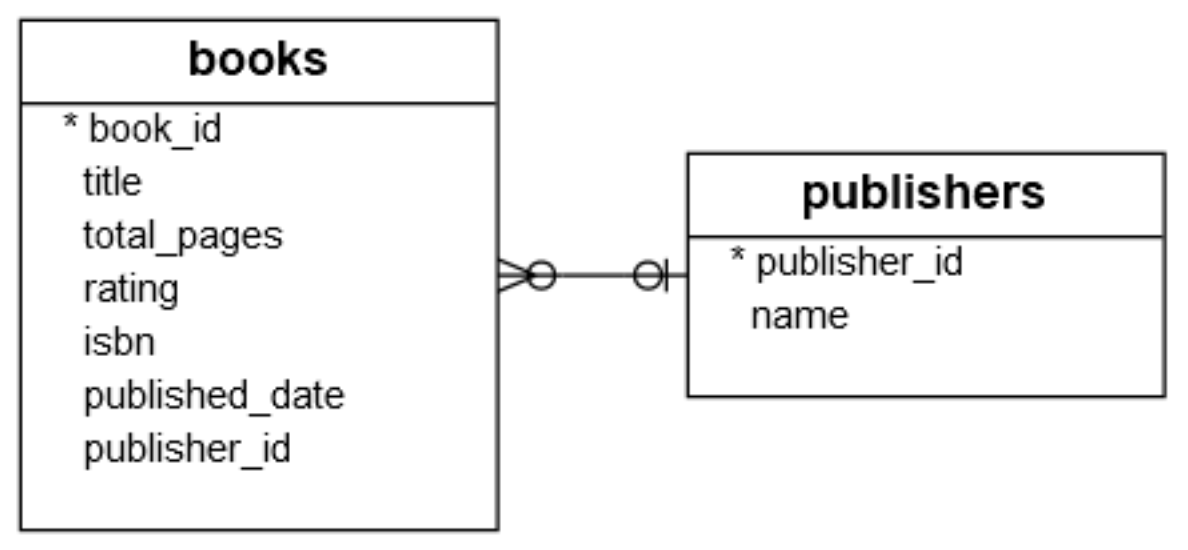
\includegraphics[scale=0.8]{screenshots/problem5.png}
    \label{fig:my_label1}
\end{figure}

\subsection*{A publisher may have zero or many books while a book may belong to zero or one publisher. The relationship between the books table and the publishers table is zero-to-many.
Based on the information given above, write queries for the following: }

\subsubsection*{(a) A query which will return information about books with publishers, irrespective of whether a book
has associated publishers or not.}

\fbox{ 
    \begin{minipage}{40em}
    \inputminted{mysql}{src/5a.sql}
    \end{minipage}
}

\subsubsection*{(b) A query which will return information about books with publishers, irrespective of whether the
publisher has any published books or not.}

\fbox{ 
    \begin{minipage}{40em}
    \inputminted{mysql}{src/5b.sql}
    \end{minipage}
}

\newpage

\end{document}